% =============================================================================
% NUS AI-Know Generated Presentation - Part 1 to 3
% Compile with: lualatex your_filename.tex
% =============================================================================
\documentclass[aspectratio=169]{beamer}
\usepackage{beamerthememidcenturymodern}
\usepackage[backend=biber, style=authoryear, sorting=nyt]{biblatex}
\addbibresource{demo.bib} % Assumes your bib file is named demo.bib

% --- Theme selection ---
\mcmTheme{Kraft}

% --- Metadata ---
\institute{Singapore Nuclear Research and Safety Institute}

\titlegraphic{
  \begin{minipage}{0.21\linewidth}
    \begin{center}

    \end{center}
  \end{minipage}
}


% --- Automatic section/subsection pages ---
\AtBeginSection[]{%
  \begin{frame}[plain]
    \sectionpage
  \end{frame}
}
\AtBeginSubsection[]{%
  \begin{frame}[plain]
    \subsectionpage
  \end{frame}
}

\AtEveryCite{\color{mcmPrimary}}

\usepackage{graphicx}
\usepackage{amsmath}
\usepackage{booktabs}
\usepackage{float}

% --- Title Information (Revised) ---
\title[Controlling a Nuclear Reactor]{Powering the Nation: Can You Control a Nuclear Reactor?}
\subtitle{An Introduction to Reactor Safety \& Dynamics}
\author{Dr Theodore Ong, SNRSI, NUS}
\date{\today}

\begin{document}

% =============================================================================
% PART 1: THE HOOK - "YOU ARE THE OPERATOR"
% =============================================================================

% --- Slide 1: Title Slide ---
\begin{frame}
	\titlepage
\end{frame}

% --- Slide 2: The Singapore Context ---
\begin{frame}[allowframebreaks]{The Big Question: Powering Singapore's Future}
    Singapore faces a major challenge known as the \textbf{Energy Trilemma}:

    \vspace{1.5em}
    \begin{columns}[T]
        \begin{column}{0.33\textwidth}
            \centering
            \Large \textbf{Secure}
            \vspace{0.5em}
            \normalsize Can we guarantee a stable supply that never fails?
        \end{column}
        \begin{column}{0.33\textwidth}
            \centering
            \Large \textbf{Affordable}
            \vspace{0.5em}
            \normalsize Can we keep electricity costs low for everyone?
        \end{column}
        \begin{column}{0.33\textwidth}
            \centering
            \Large \textbf{Sustainable}
            \vspace{0.5em}
            \normalsize Can we generate power without contributing to climate change?
        \end{column}
    \end{columns}

    \vspace{2em}
    \begin{block}{A Potential Solution?}
        Advanced nuclear reactors are being considered globally as a high-tech solution that could potentially address all three points. But are they safe?
	\end{block}
\end{frame}

% --- Slide 3: The Mission Briefing ---
\begin{frame}[allowframebreaks]{Your Mission, Should You Choose to Accept It}
    \begin{columns}
        \begin{column}{0.6\textwidth}
            Today, you are not just students. You are reactor operators at the controls of a next-generation Fluoride-salt-cooled High-temperature Reactor (FHR).

            \vspace{1em}

            \textbf{The Situation:}
            The grid operator requests an immediate increase in power output to meet a sudden demand spike.

            \vspace{1em}

            \begin{alertblock}{Your Objective}
                Increase reactor thermal power from \textbf{30 MWth} to \textbf{60 MWth} and stabilize it there.
            \end{alertblock}
        \end{column}
        \begin{column}{0.4\textwidth}
            \centering
			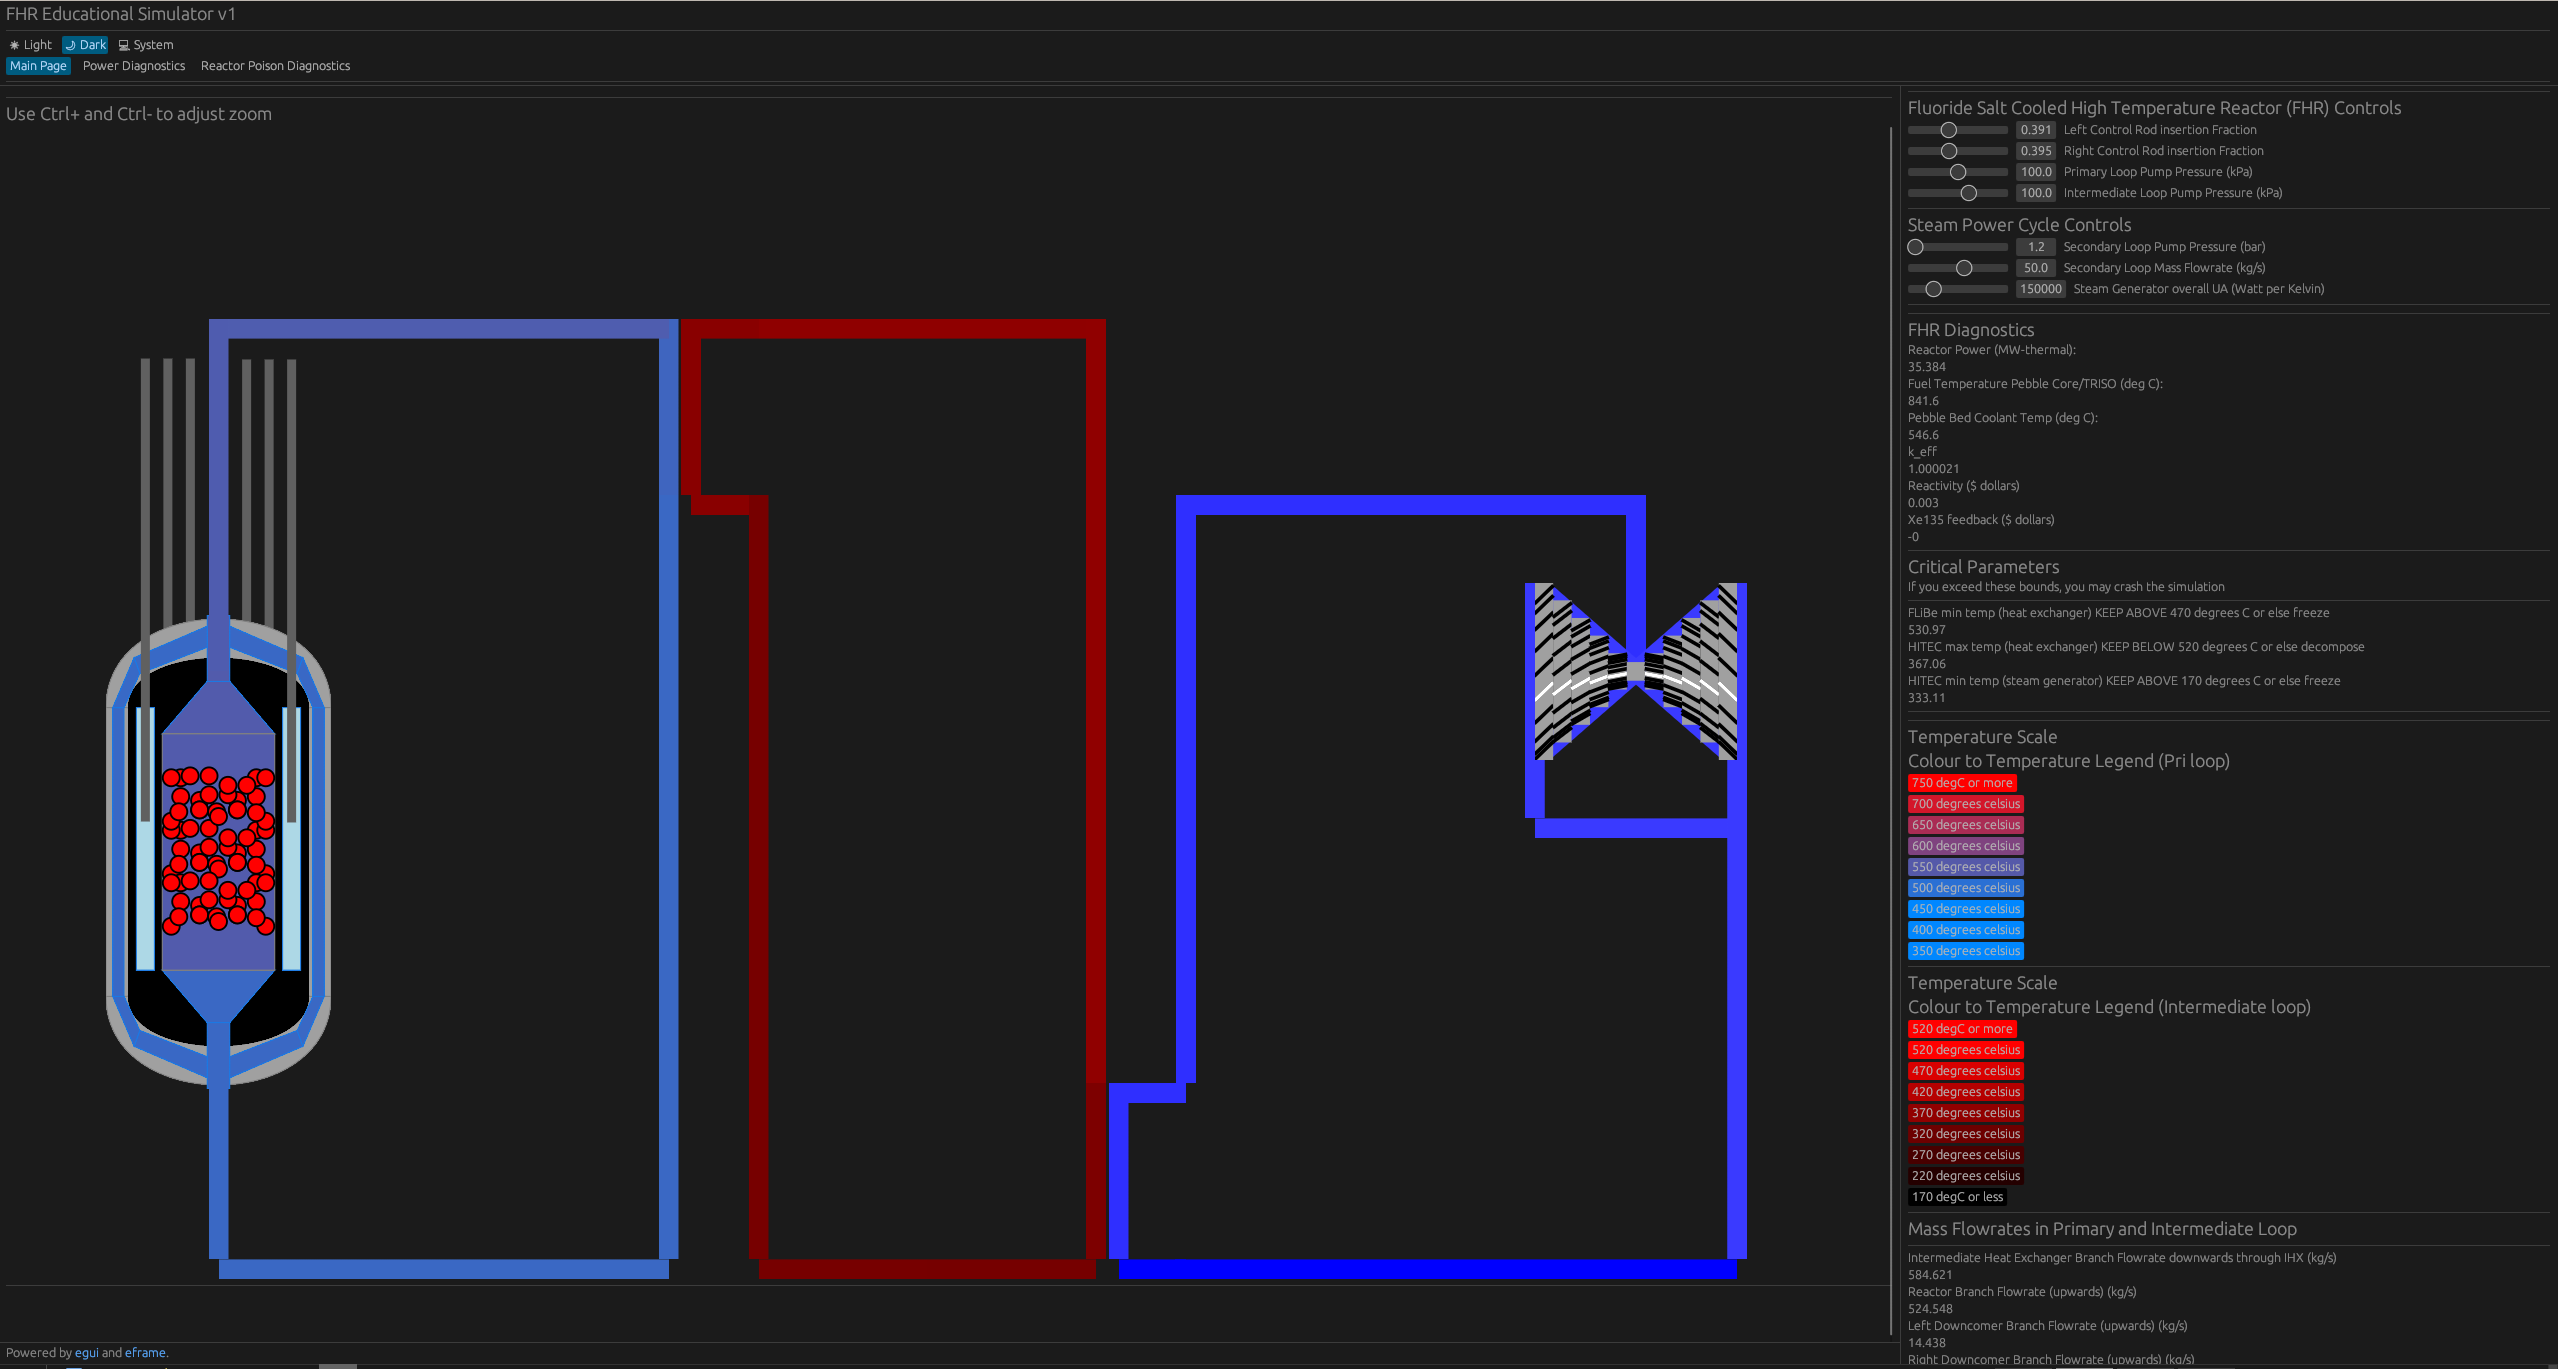
\includegraphics[width=0.8\textwidth]{./fhr_sim_full.png}
        \end{column}
    \end{columns}
\end{frame}

% --- Slide 4: Operational Constraints ---
\begin{frame}[allowframebreaks]{Operational Constraints \& Safety Limits}
    Nuclear reactors are powerful systems that require precise control. We cannot just "floor the accelerator."

    \vspace{1em}

    \textbf{The Rules of Engagement:}
    \begin{itemize}
        \item You have full control over the reactor's control rods (reactivity).
        \item You must aim for exactly \textbf{60 MWth}.
    \end{itemize}

    \vspace{2em}

    \begin{block}{SAFETY LIMIT (FAILURE CONDITION)}
        If reactor power exceeds \textbf{1000 MWth} at any point during the maneuver, you have violated the reactor's safety limits and failed the mission.
    \end{block}
\end{frame}

% =============================================================================
% PART 2: THE INTERACTIVE CHALLENGE
% =============================================================================

% --- Slide 5: Simulator Interface Overview ---
\begin{frame}[allowframebreaks]{Your Interface: The FHR Control Panel}
	\begin{figure}[H]
		\centering
		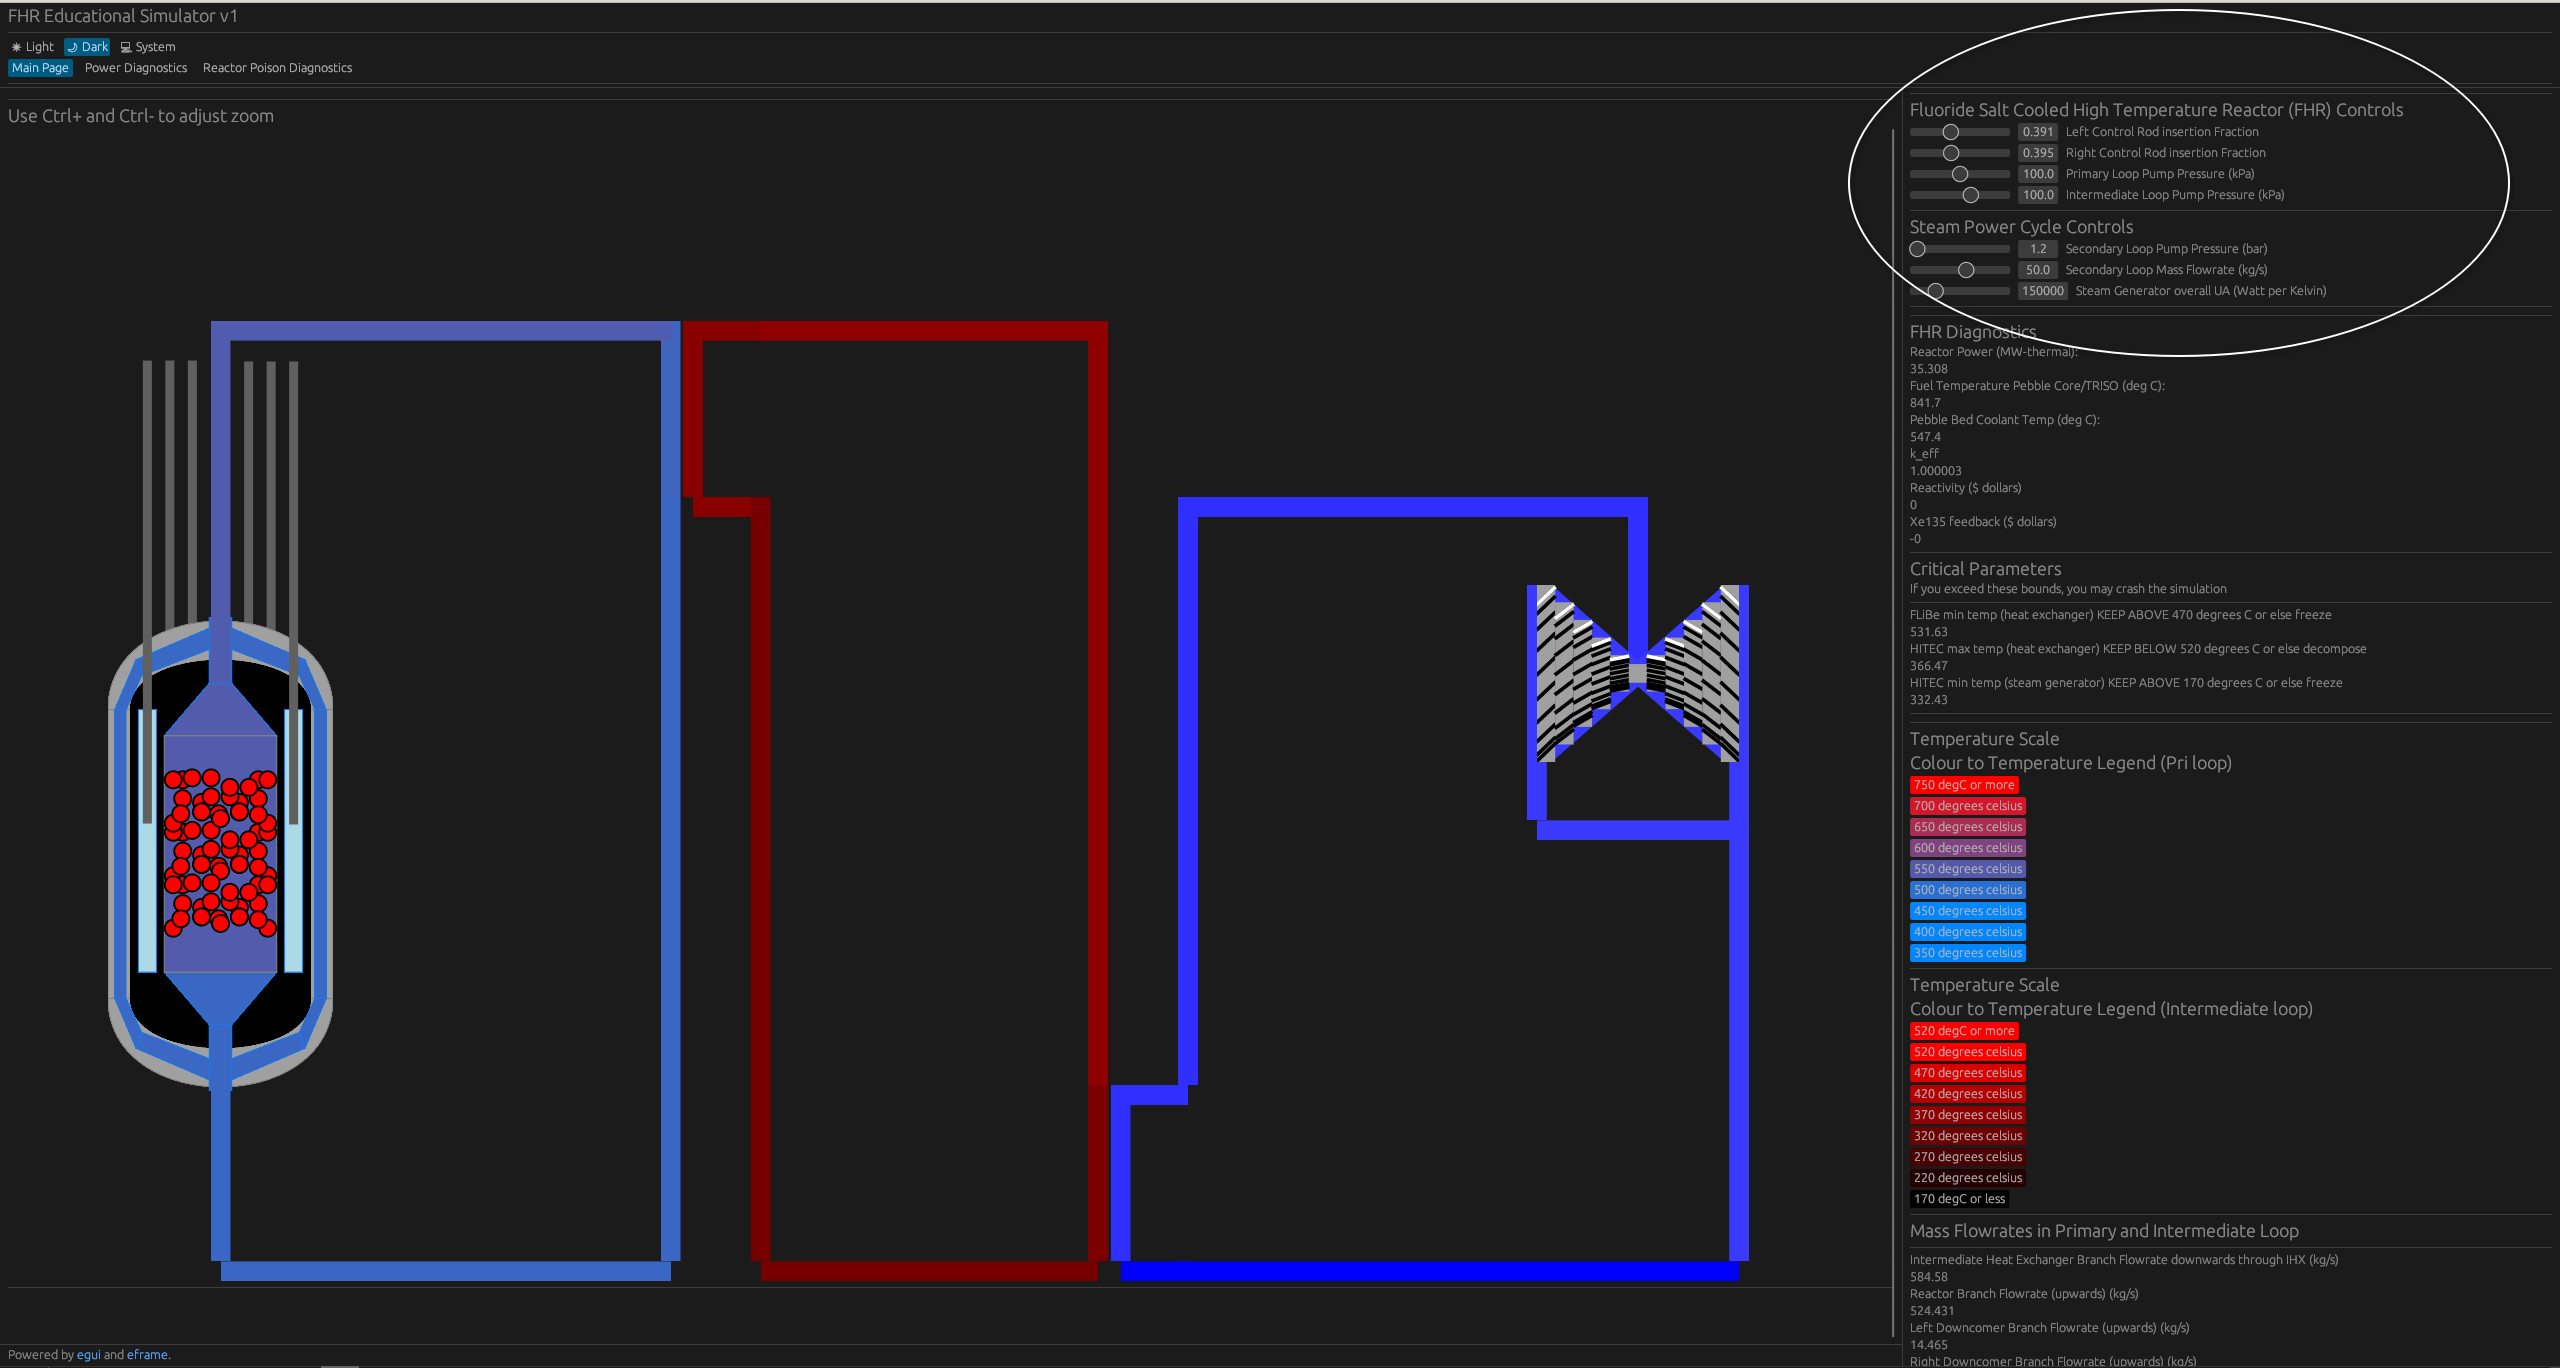
\includegraphics[width=0.7\textwidth, keepaspectratio]{./fhr_sim_controls.png}
		\caption{\textit{Current State: Stable at 30 MWth} }
		\label{fig:fhr-controls} % Optional: for cross-referencing later
	\end{figure}
\end{frame}

% --- New Slide: The Individual Challenge ---
\begin{frame}[allowframebreaks]{The Challenge: Solve it at Your Desk}
    You've seen the controls and you know the mission. Now it's your turn to try and crack the problem.

    \vspace{1.5em}

    \begin{block}{Your Task (5 Minutes)}
        On your own computer, launch the simulator and attempt the power increase from \textbf{30 MWth to 60 MWth}.
        \begin{itemize}
            \item Your goal is to find a strategy to hit the target and stabilize the power.
            \item Pay close attention to how much you move the controls and for how long.
        \end{itemize}
    \end{block}

    \vspace{1.5em}

    \begin{alertblock}{Think You've Cracked It?}
        If you figure out a successful technique, get ready! In a few minutes, I will be asking for volunteers to come up and demonstrate their solution on the main screen in front of the class.
    \end{alertblock}

    \vspace{1em}
    \centering
    \Large\textbf{Your time starts now!}
\end{frame}

% --- Slide 6: The Challenge Begins ---
\begin{frame}[allowframebreaks]{The Challenge Begins}
    \centering
    \Huge \textbf{Volunteers Needed!}

    \vspace{2em}
    \normalsize
    Who has the steady hand to bring us to 60 MWth without exceeding 1000 MWth?

    \vspace{2em}
    \hrule
    \vspace{1em}

    \textbf{For the rest of the class (Observers):}
    Watch closely. Don't just look at the power level.
    \begin{itemize}
        \item How does the reactor respond immediately after they move the controls?
        \item What happens to the power when they \textit{stop} moving the controls?
        \item Does the reactor feel "heavy" (slow to move) or "twitchy" (fast to move)?
    \end{itemize}
\end{frame}

% --- Slide 7: Debrief ---
\begin{frame}[allowframebreaks]{Debrief: Intuition vs. Reality}
    It wasn't as easy as turning up a volume knob on a radio.

    \vspace{1em}

    \textbf{Discussion Questions:}
    \begin{enumerate}
        \item Did anyone overshoot the 60 MWth target? Why do you think that happened?
        \item Did you notice the power continuing to change even after the controls were put back to neutral?
        \item If you added too much reactivity, did it feel like the reactor was "running away" from you?
    \end{enumerate}

    \vspace{1em}
    \begin{center}
        \textbf{Why does the reactor have "momentum"? Why doesn't it stop instantly?}
        
        \textit{To answer this, we need to understand what makes nuclear engineering a unique challenge.}
    \end{center}
\end{frame}

% =============================================================================
% PART 3: BRIDGING THE GAP FROM SIMPLICITY TO REALITY
% =============================================================================

% --- Slide 8: Is It Really That Simple? ---
\begin{frame}[allowframebreaks]{Is It Really That Simple?}
    On paper, the concept of a nuclear reactor sounds straightforward:
    
    \vspace{1.5em}
    \begin{center}
        \textit{"Neutrons split uranium to heat something that then boils water to spin a turbine."}
    \end{center}
    \vspace{1.5em}

    But you just experienced it for yourselves. It wasn't that simple.
    \begin{itemize}
        \item The power had "momentum."
        \item It was easy to overshoot the target.
        \item It didn't respond like a car engine or a volume knob.
    \end{itemize}

    \vspace{1.5em}
    \begin{exampleblock}{The Core Question}
        If the basic idea is so easy, why is controlling it so tricky?
        
        The gap between that simple sentence and a safe, working power plant is precisely why nuclear science and engineering is such a deep and fascinating field.
    \end{exampleblock}
\end{frame}

% --- Slide 9: The Journey from Paper to Power Plant ---
\begin{frame}[allowframebreaks]{The Journey from Paper to Power Plant}
    To use nuclear energy to help solve Singapore's energy trilemma, we must bridge that gap.
    
    \vspace{1em}
    \textbf{How do we get from a paper design to a safe, working plant that can operate for 60+ years?}
    
    \vspace{1em}
    It's a grand challenge with many layers:
    \begin{itemize}
        \item \textbf{Politics \& Public Policy:} How do we regulate and govern this technology?
        \item \textbf{Economics \& Finance:} How do we fund and build such a large project?
        \item \textbf{Social Acceptance:} How do we ensure public trust and communicate effectively?
        \item \textbf{Technical \& Engineering Safety:} How do we guarantee the plant will be safe under all possible conditions?
    \end{itemize}
    
    \vspace{1em}
    \begin{alertblock}{Our Focus Today: Technical Safety}
        My work, and what we'll explore next, lives in that last box. This is the world of \textbf{Reactor Safety}, where we must understand every physical process inside the core.
    \end{alertblock}
\end{frame}

% =============================================================================
% PART 4: A TOUR OF THE PHENOMENA WE MUST MASTER (REVISED)
% =============================================================================

% --- Slide 10: Introduction to the Tour ---
\begin{frame}[allowframebreaks]{What Phenomena Do We Study?}
    To guarantee safety, we can't just have a good design on paper. We have to understand, predict, and master every single physical process happening inside the reactor.

    \vspace{1.5em}
    We call these the core \textbf{phenomena}.
    
    \vspace{1.5em}
    \begin{block}{A Tour of the Frontier}
        Let's take a quick tour of the four most critical areas that reactor safety engineers and scientists spend their careers studying.
    \end{block}
\end{frame}

% --- Slide 11: Phenomenon #1: Neutronics ---
\begin{frame}[allowframebreaks]{Phenomenon \#1: Neutronics - The Engine of the Reactor}
    \textbf{Concept:} Neutronics is the study of the neutron population in the reactor. This population directly determines the reactor's power level, generating about 90\% of the heat during operation.

    \vspace{1em}
    \textbf{The Safety Question:} How do we precisely predict and control the neutron population to generate steady power and ensure the chain reaction never runs away?

    \vspace{1.5em}
    \begin{exampleblock}{From Simple Models to Reality}
        For basic control dynamics—the "momentum" you felt—we can use the \textbf{Point Reactor Kinetics Equations (PRKE)}.
        \begin{itemize}
            \item It simplifies the entire reactor down to a single point in space.
            \item \textbf{The FHR simulator you used runs on the 6-group PRKE model} to accurately capture the effect of delayed neutrons.
        \end{itemize}
        \vspace{1em}
        However, true neutron behavior is far more complex. To design a reactor, we must account for:
        \begin{itemize}
            \item \textbf{Where} neutrons are in the reactor (Spatial effects)
            \item \textbf{What direction} they are traveling (Angular effects)
            \item \textbf{How fast} they are moving (Energy effects)
        \end{itemize}
        This is all described by the Neutron Transport Equation, a much more complicated model that forms the basis of modern reactor physics.
    \end{exampleblock}
\end{frame}

% --- Slide 12: Phenomenon #2: Decay Heat (UPDATED ANALOGY) ---
\begin{frame}[allowframebreaks]{Phenomenon \#2: Decay Heat - The Fire That Won't Go Out}
    \textbf{Concept:} The other 10\% of the reactor's heat comes from a different source. Even after you completely stop the chain reaction, the core continues to produce heat from the radioactive decay of its waste products.
    
    \vspace{1em}
    \textbf{Think of it like a cooker stove with a unique problem: you can turn the knob to "off" to stop the main flame, but you cannot turn off the burner completely. It continues to generate heat no matter what.}
    
    \vspace{1em}
    \begin{block}{A Real-World Example: Fukushima}
        The reactors at Fukushima Daiichi shut down perfectly when the earthquake hit. The meltdowns were caused by the failure to remove this powerful \textbf{decay heat} after the tsunami destroyed the cooling pumps.
    \end{block}

    \vspace{1em}
    \textbf{The Safety Question:} How do we design systems that can remove this residual heat reliably, even if all power is lost? This leads us directly to our next challenge...
\end{frame}



% --- Slide 13: Phenomenon #3: Heat Transfer ---
\begin{frame}[allowframebreaks]{Phenomenon \#3: Heat Transfer - The Cooling Challenge}
    \textbf{Concept:} Heat transfer is about moving heat from where it's produced (the fuel) to where it can be used (the turbine). This involves two major challenges.

    \vspace{1em}
    \begin{alertblock}{Problem 1: Avoiding Overheating (in Water-Cooled Reactors)}
        In Pressurized and Boiling Water Reactors (PWRs/BWRs), if the fuel gets too hot, the water can form a steam blanket around it (Critical Heat Flux). This blocks cooling and can lead to fuel damage.
    \end{alertblock}
    
    \vspace{1em}
    \begin{exampleblock}{Problem 2: Ensuring Coolant Flow (in All Reactors)}
        To remove decay heat and prevent a Fukushima-like event, we must keep the coolant circulating.
        \begin{itemize}
            \item \textbf{Forced Circulation:} Uses pumps. Powerful and controllable, but requires electricity.
            \item \textbf{Natural Circulation:} Uses physics (hot coolant rises, cool coolant sinks). It is passive and highly reliable, operating without any pumps or external power.
        \end{itemize}
        Modern advanced reactors are designed to have strong natural circulation capabilities as a core safety feature.
    \end{exampleblock}
    
    \textit{Note: For HTGRs, FHRs, and MSRs, which use single-phase coolants (gas or liquid salt), Critical Heat Flux is not a concern, allowing them to operate at higher temperatures and focus on the circulation problem.}
\end{frame}

% --- NEW SLIDE 14: Experimental CHF Testing ---
\begin{frame}[allowframebreaks]{Case Study: Testing Heat Transfer Without a Reactor}
    To study complex phenomena like Critical Heat Flux, we don't need a real reactor. We can build sophisticated non-nuclear test facilities.
    
    \begin{columns}[T]
        \begin{column}{0.5\textwidth}
            \begin{block}{How It Works}
                Instead of nuclear fuel, we use precisely machined \textbf{electric heater rods}.
                \begin{itemize}
                    \item These rods can be powered to perfectly mimic the heat output of actual fuel.
                    \item This is far safer, cheaper, and allows for detailed measurements.
                    \item We can study complex effects, like how the rocking motion of a ship might affect CHF on a marine reactor \cite{ku2026experimental}.
                \end{itemize}
            \end{block}
        \end{column}
        \begin{column}{0.5\textwidth}
            \begin{figure}[H]
                \centering
                % Placeholder for an image of a CHF test loop
                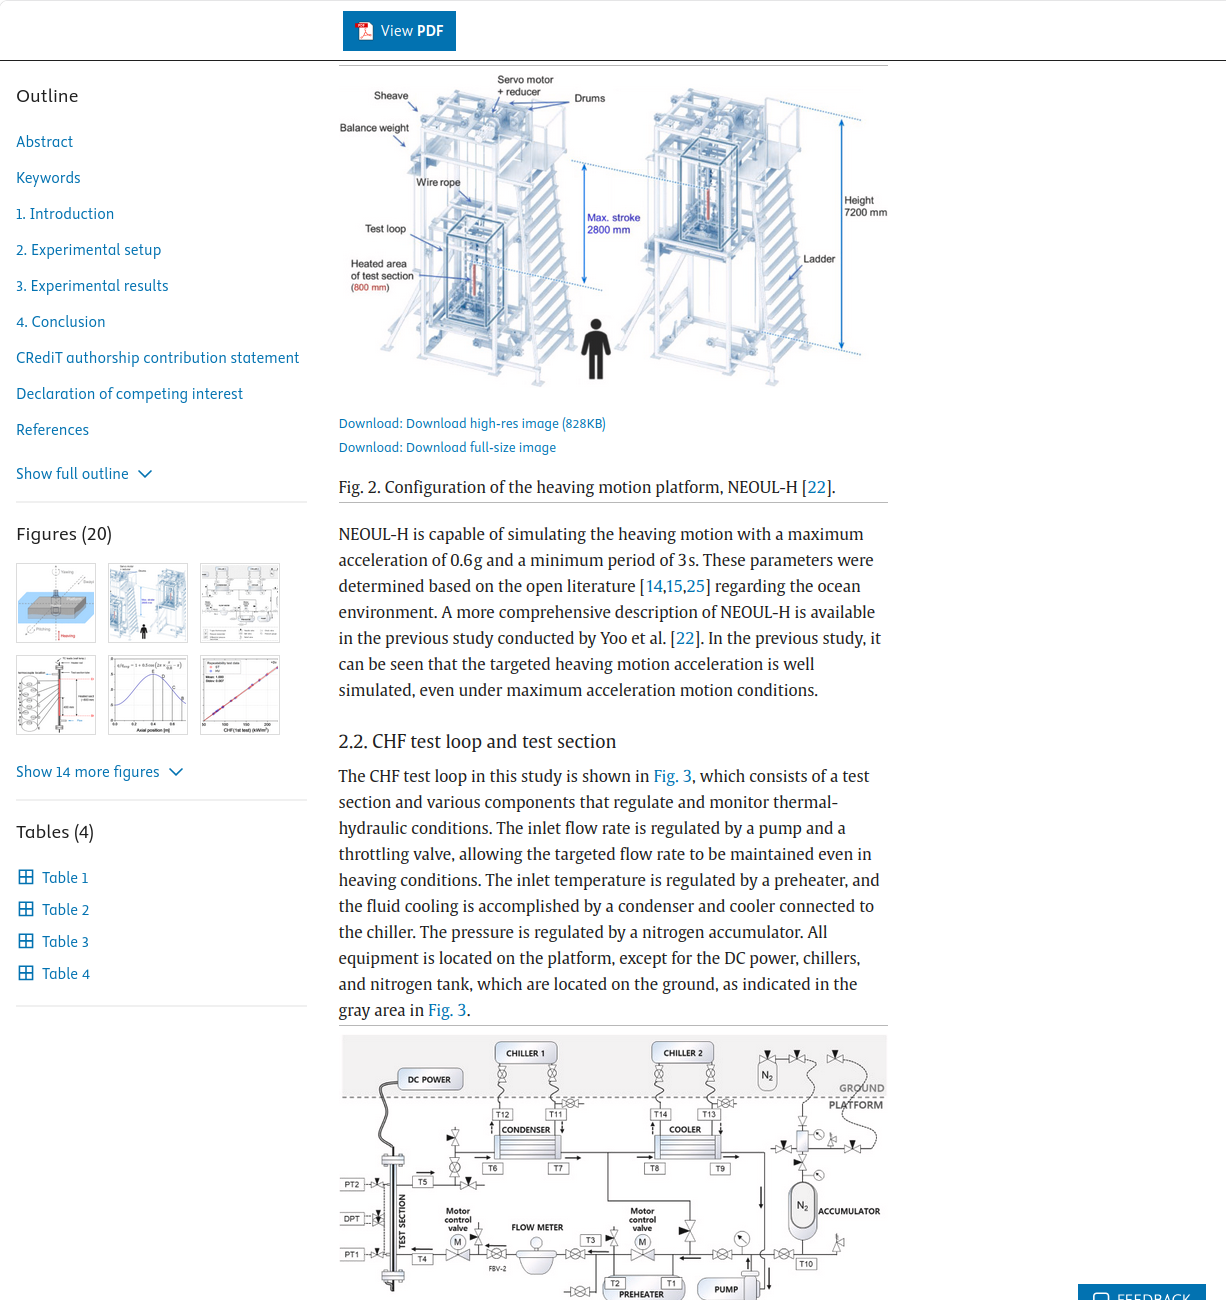
\includegraphics[width=\textwidth, keepaspectratio]{chf_expt_setup.png}
                \caption{An example of an experimental loop for studying flow boiling phenomena.}
            \end{figure}
        \end{column}
    \end{columns}
\end{frame}

% --- Slide: Case Study: Testing Natural Circulation with CIET ---
\begin{frame}[allowframebreaks]{Case Study: Testing Natural Circulation with CIET}
    For system-wide behavior like natural circulation, we build "Integral Effects Test" (IET) facilities that model the entire reactor loop.
	\begin{figure}[H]
		\centering
				% Placeholder for your CIET simulator image
		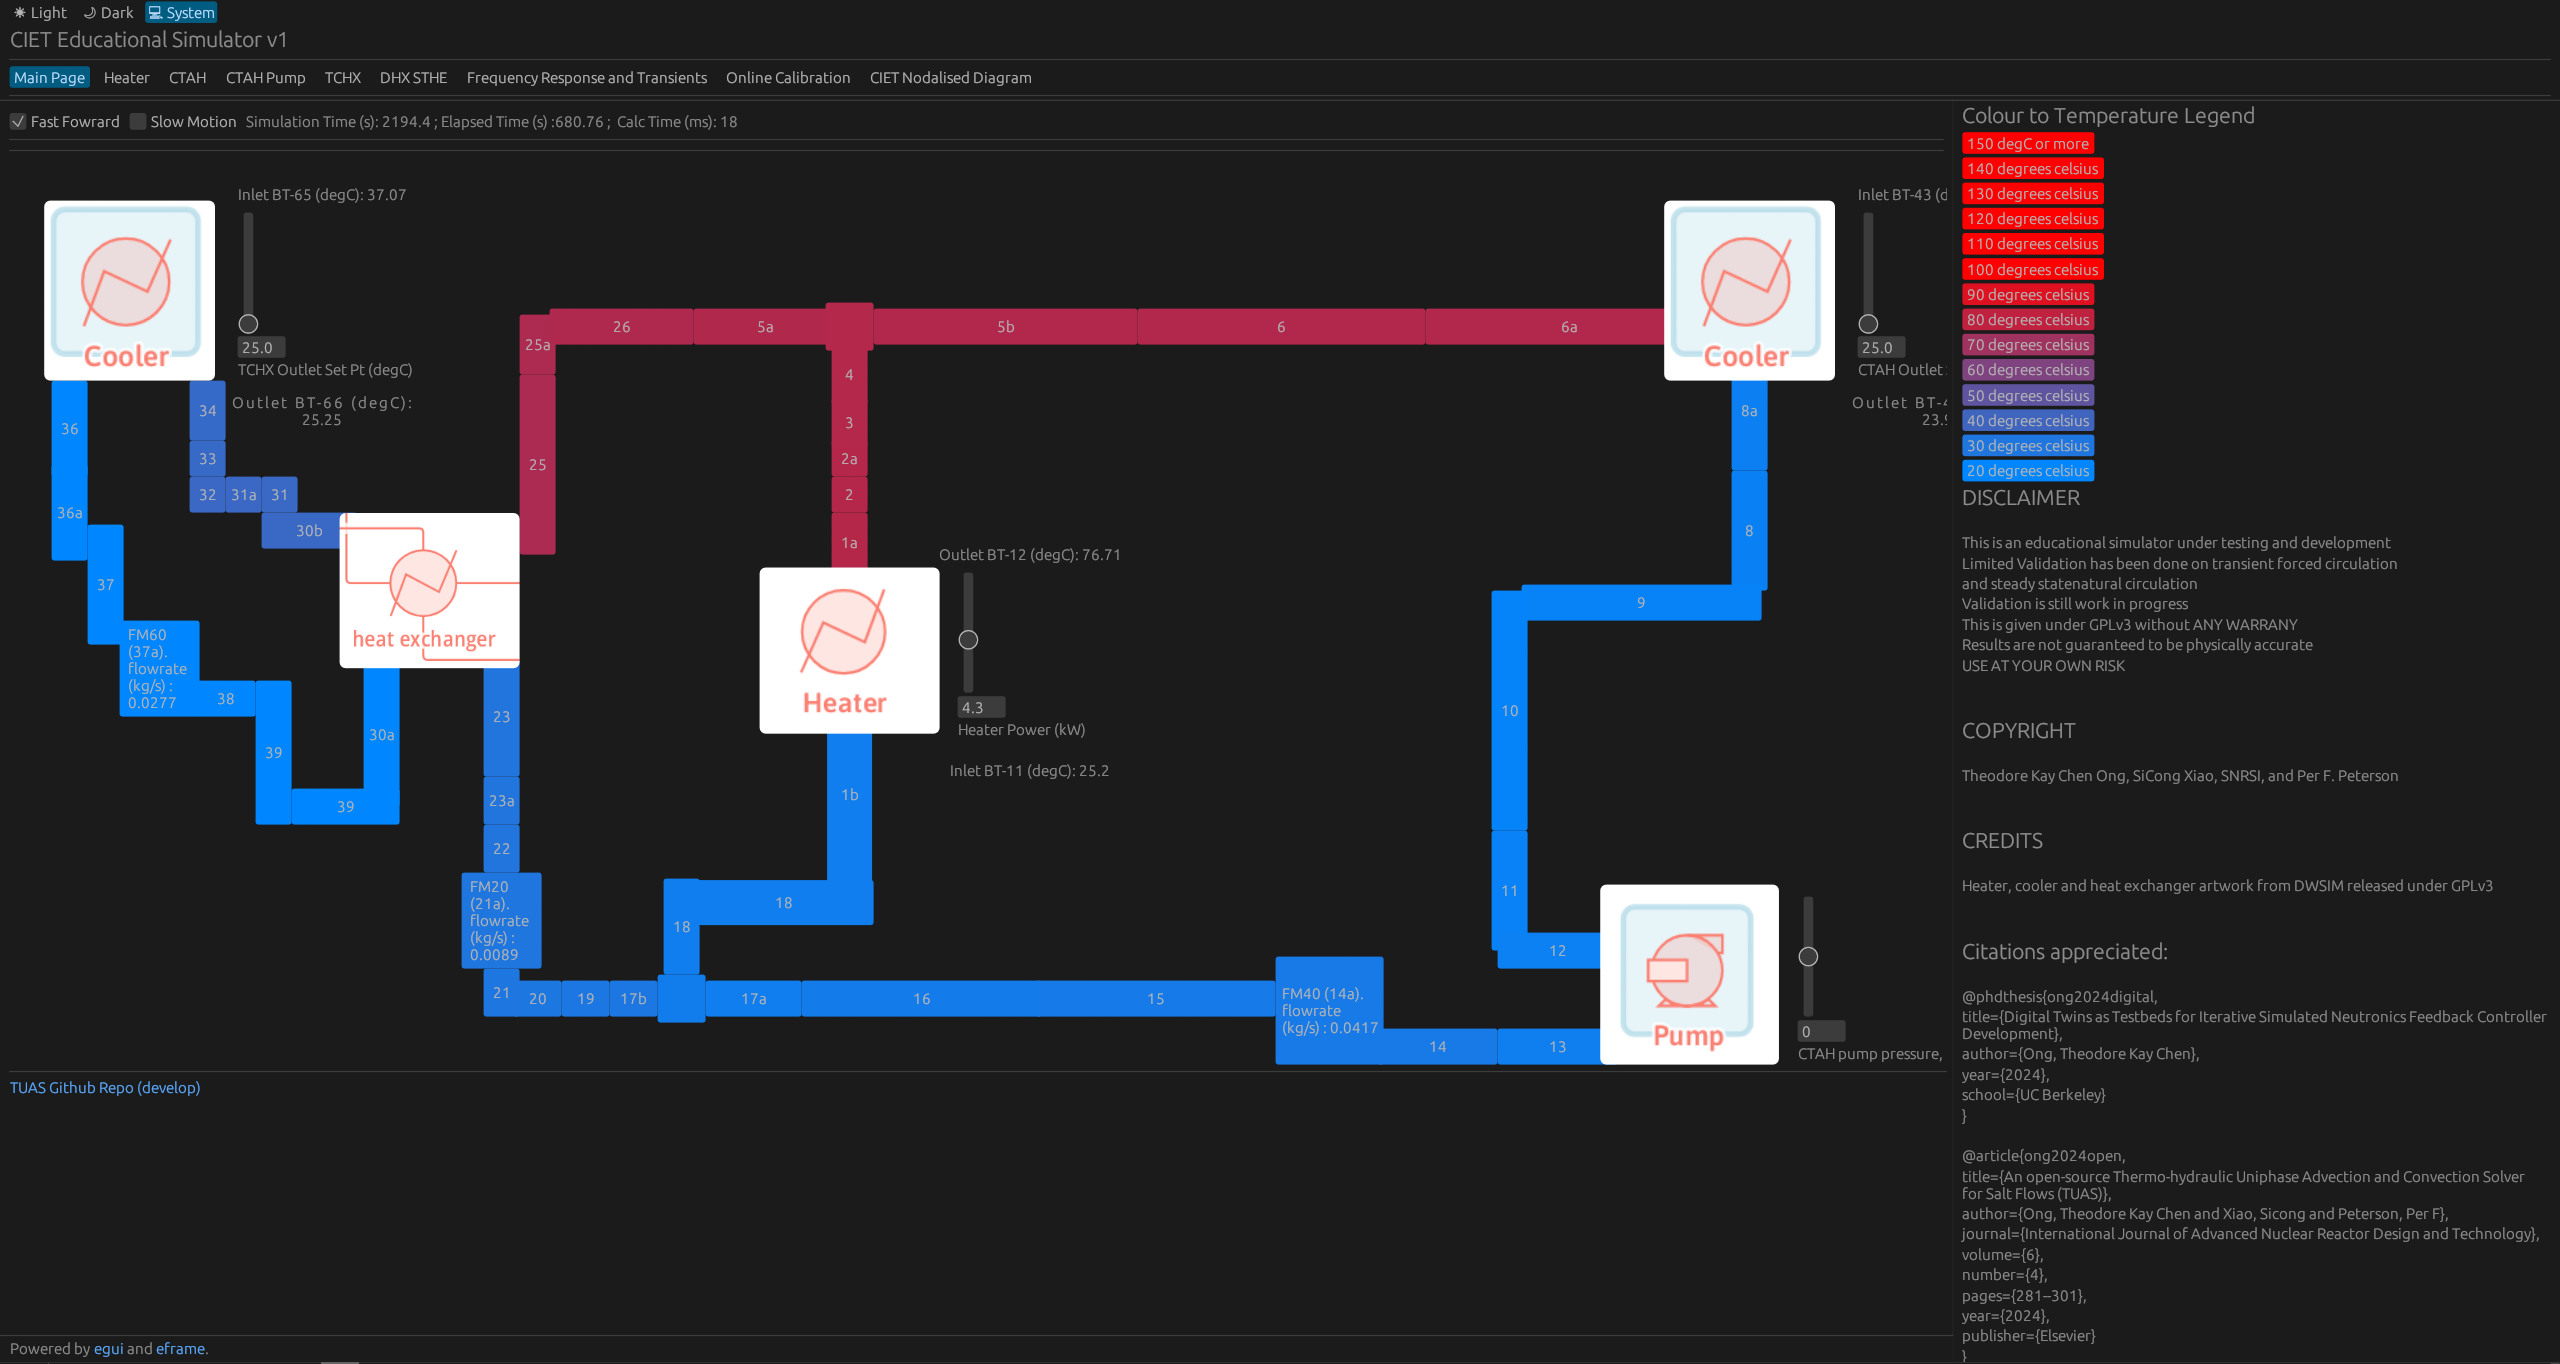
\includegraphics[width=0.8\textwidth, keepaspectratio]{ciet_simulator.png}
		\caption{The Compact Integral Effects Test (CIET) Educational Simulator.}
	\end{figure}
\end{frame}
\begin{frame}[allowframebreaks]{Case Study: Testing Natural Circulation with CIET}
    For system-wide behavior like natural circulation, we build "Integral Effects Test" (IET) facilities that model the entire reactor loop.
	\begin{alertblock}{The Limits of Natural Circulation}
		It is a powerful passive safety feature, but it has challenges:
		\begin{itemize}
			\item \textbf{Lower Flow Rate:} The flow is inherently weaker than with pumps, so heat removal is slower.
			\item \textbf{Flow Instability:} The flow can become unstable and oscillate, which can hamper heat removal.
			\item \textbf{CHF is Still a Risk:} In water systems, we must prove that the weaker natural flow is still fast enough to prevent a CHF event.
		\end{itemize}
	\end{alertblock}
\end{frame}

% --- Slide 15: Phenomenon #4: Materials Science (Part 1) ---
\begin{frame}[allowframebreaks]{Phenomenon \#4: Materials Science - Fuel \& Vessels}
    \textbf{Concept:} The inside of a reactor is one of the most extreme environments imaginable. Materials science asks: what can we build it out of?
    \vspace{1em}
    \begin{exampleblock}{Micro-Scale: The Fuel (TRISO)}
        \begin{columns}
            \begin{column}{0.6\textwidth}
                HTGRs and FHRs use TRISO fuel. Each poppy-seed-sized particle has ceramic layers that act as a personal containment vessel, trapping radioactive products inside at temperatures up to 1600°C.
            \end{column}
            \begin{column}{0.4\textwidth}
                \centering
                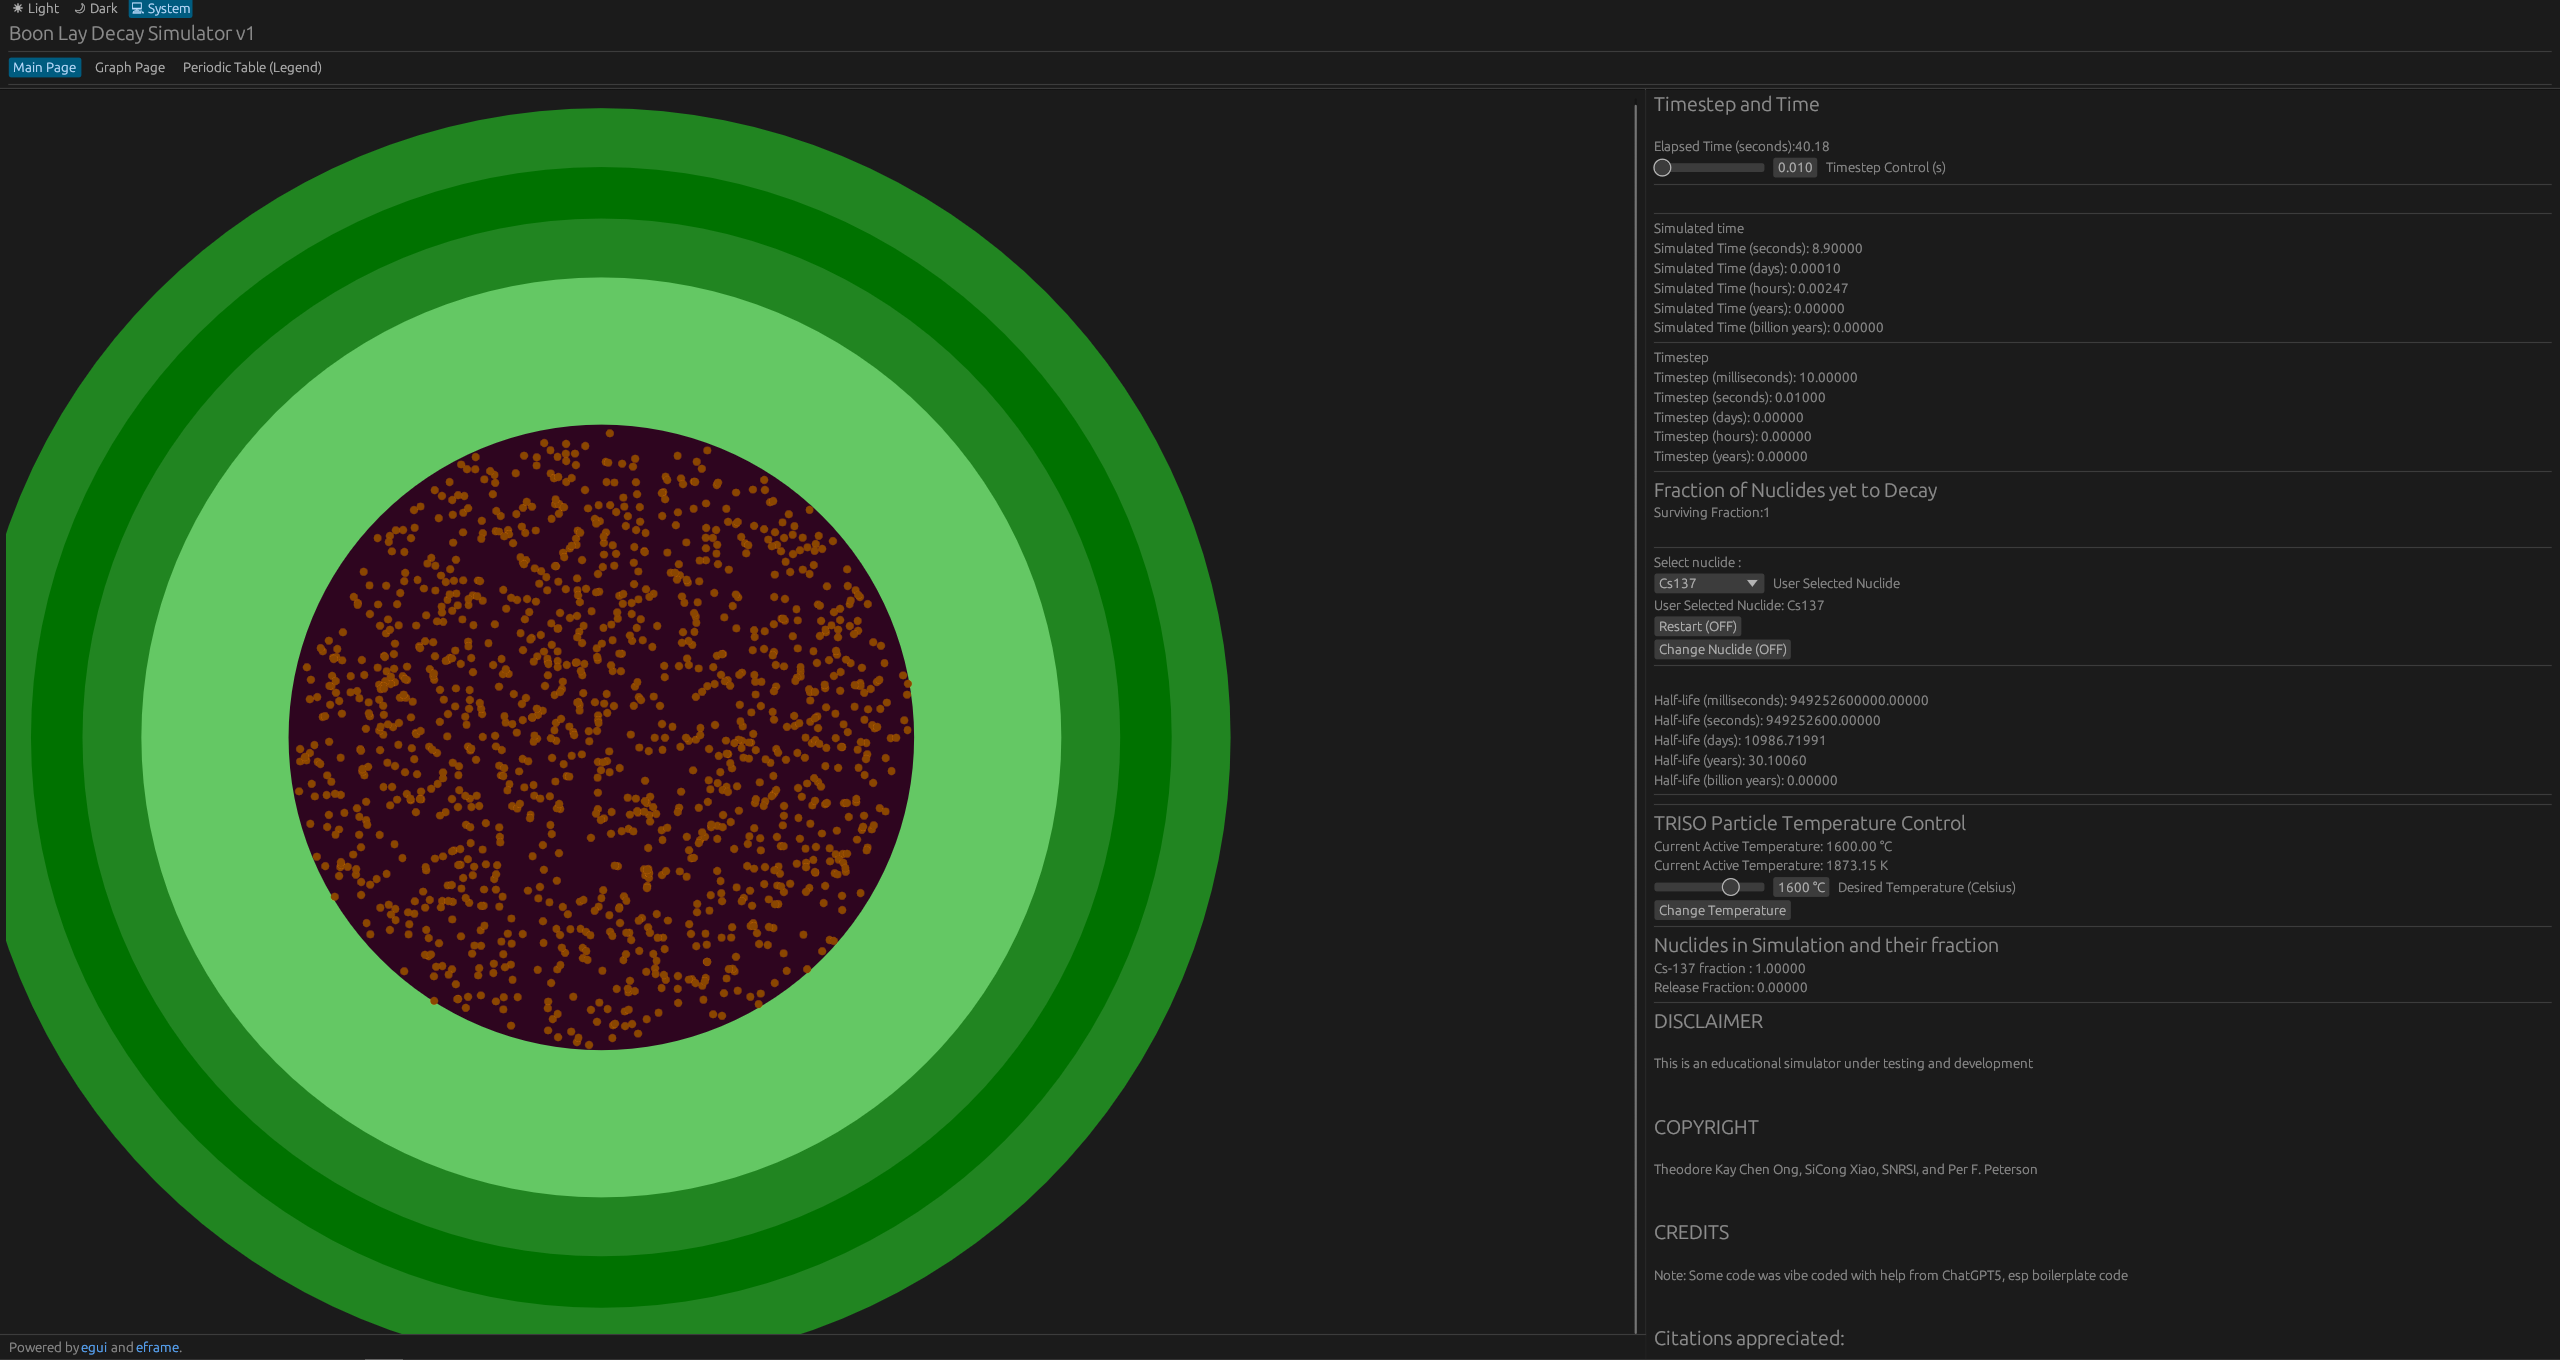
\includegraphics[width=\textwidth]{triso_particle.png}
                \tiny{Cross-section of a TRISO particle.}
            \end{column}
        \end{columns}
    \end{exampleblock}
\end{frame}

% --- NEW SLIDE 16: Materials Science (Part 2) ---
\begin{frame}[allowframebreaks]{Phenomenon \#4 (cont.): The Challenge of Steel Vessels}
    \textbf{The Safety Question:} How do we ensure the massive steel Reactor Pressure Vessel (RPV), which contains the entire core, remains intact for over 60 years?
    \begin{columns}[T]
        \begin{column}{0.5\textwidth}
            \begin{figure}[H]
                \centering
				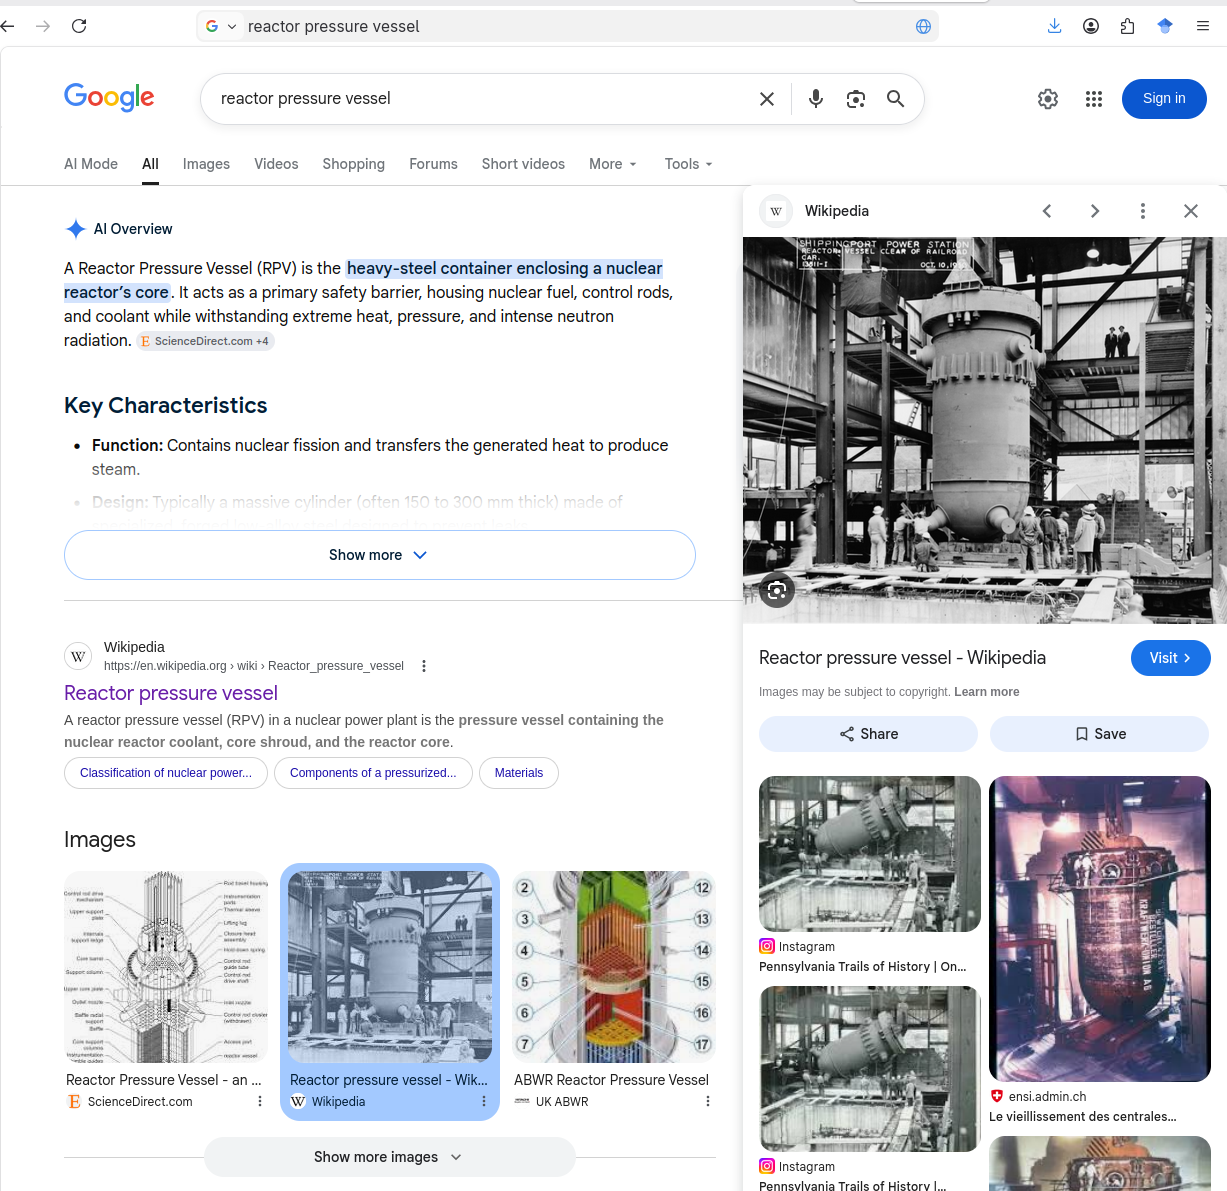
\includegraphics[width=0.7\textwidth, keepaspectratio]{rpv_image.png}
                \caption{Just a simple Google for RPV pictures}
            \end{figure}
        \end{column}
        \begin{column}{0.5\textwidth}
            \begin{alertblock}{Engineers must prevent failures from:}
                \begin{itemize}
                    \item \textbf{Brittle Fracture:} Radiation can make steel brittle like glass. We must ensure it always remains tough and ductile.
                    \item \textbf{High Cycle Fatigue:} Repeated stress from temperature and pressure changes can cause cracks to grow over time.
                    \item \textbf{Creep:} At high temperatures, the steel can slowly and permanently deform under pressure.
                \end{itemize}
            \end{alertblock}
        \end{column}
    \end{columns}
\end{frame}

% --- NEW SLIDE 17: Phenomenon #5: Shielding & Transport ---
\begin{frame}[allowframebreaks]{Phenomenon \#5: Shielding \& Radionuclide Transport}
    \textbf{Concept:} The fission process creates intense radiation and radioactive materials. We must contain them.
	\textbf{The Safety Question:} How do we design barriers to block radiation, and how do we predict where radioactive material would go in the unlikely event of a leak?
	\begin{exampleblock}{Two Sides of the Same Coin}
		\begin{itemize}
			\item \textbf{Shielding:} Designing the massive layers of concrete, steel, and water that block radiation and protect workers and the public.
			\item \textbf{Radionuclide Transport:} Studying how radioactive materials might move through the plant or the environment in an accident scenario.
		\end{itemize}
	\end{exampleblock}
	This knowledge is essential for \textbf{Probabilistic Safety Assessment (PSA)} and for designing safe long-term \textbf{waste disposal} strategies.
\end{frame}

% =============================================================================
% FINAL SLIDES OF PART 4
% =============================================================================

% --- Slide 18: Other Areas of Study ---
\begin{frame}[allowframebreaks]{And the List Goes On...}
    Our tour has only scratched the surface. To build and operate a nuclear power plant safely, there are many other critical areas of study:
    
    \vspace{1em}
    \begin{itemize}
        \item \textbf{Power Production (Secondary Loop):} The entire non-nuclear side of the plant, including turbines, generators, and the connection to the electrical grid.
        
        \item \textbf{Process Control \& Instrumentation:} Designing the thousands of sensors and control systems that act as the reactor's nervous system.
        
        \item \textbf{Human Factors \& Human-Machine Interfaces:} Studying 
			how operators interact with the plant. A poor interface was a key 
			contributor to the Three Mile Island accident in 1979 \cite{malone1979human}
        \item And many, many more...
    \end{itemize}
\end{frame}

% --- Slide 19: Connecting Back to the Simulator ---
\begin{frame}[allowframebreaks]{Appreciating the Complexity}
    \begin{figure}[H]
        \centering
        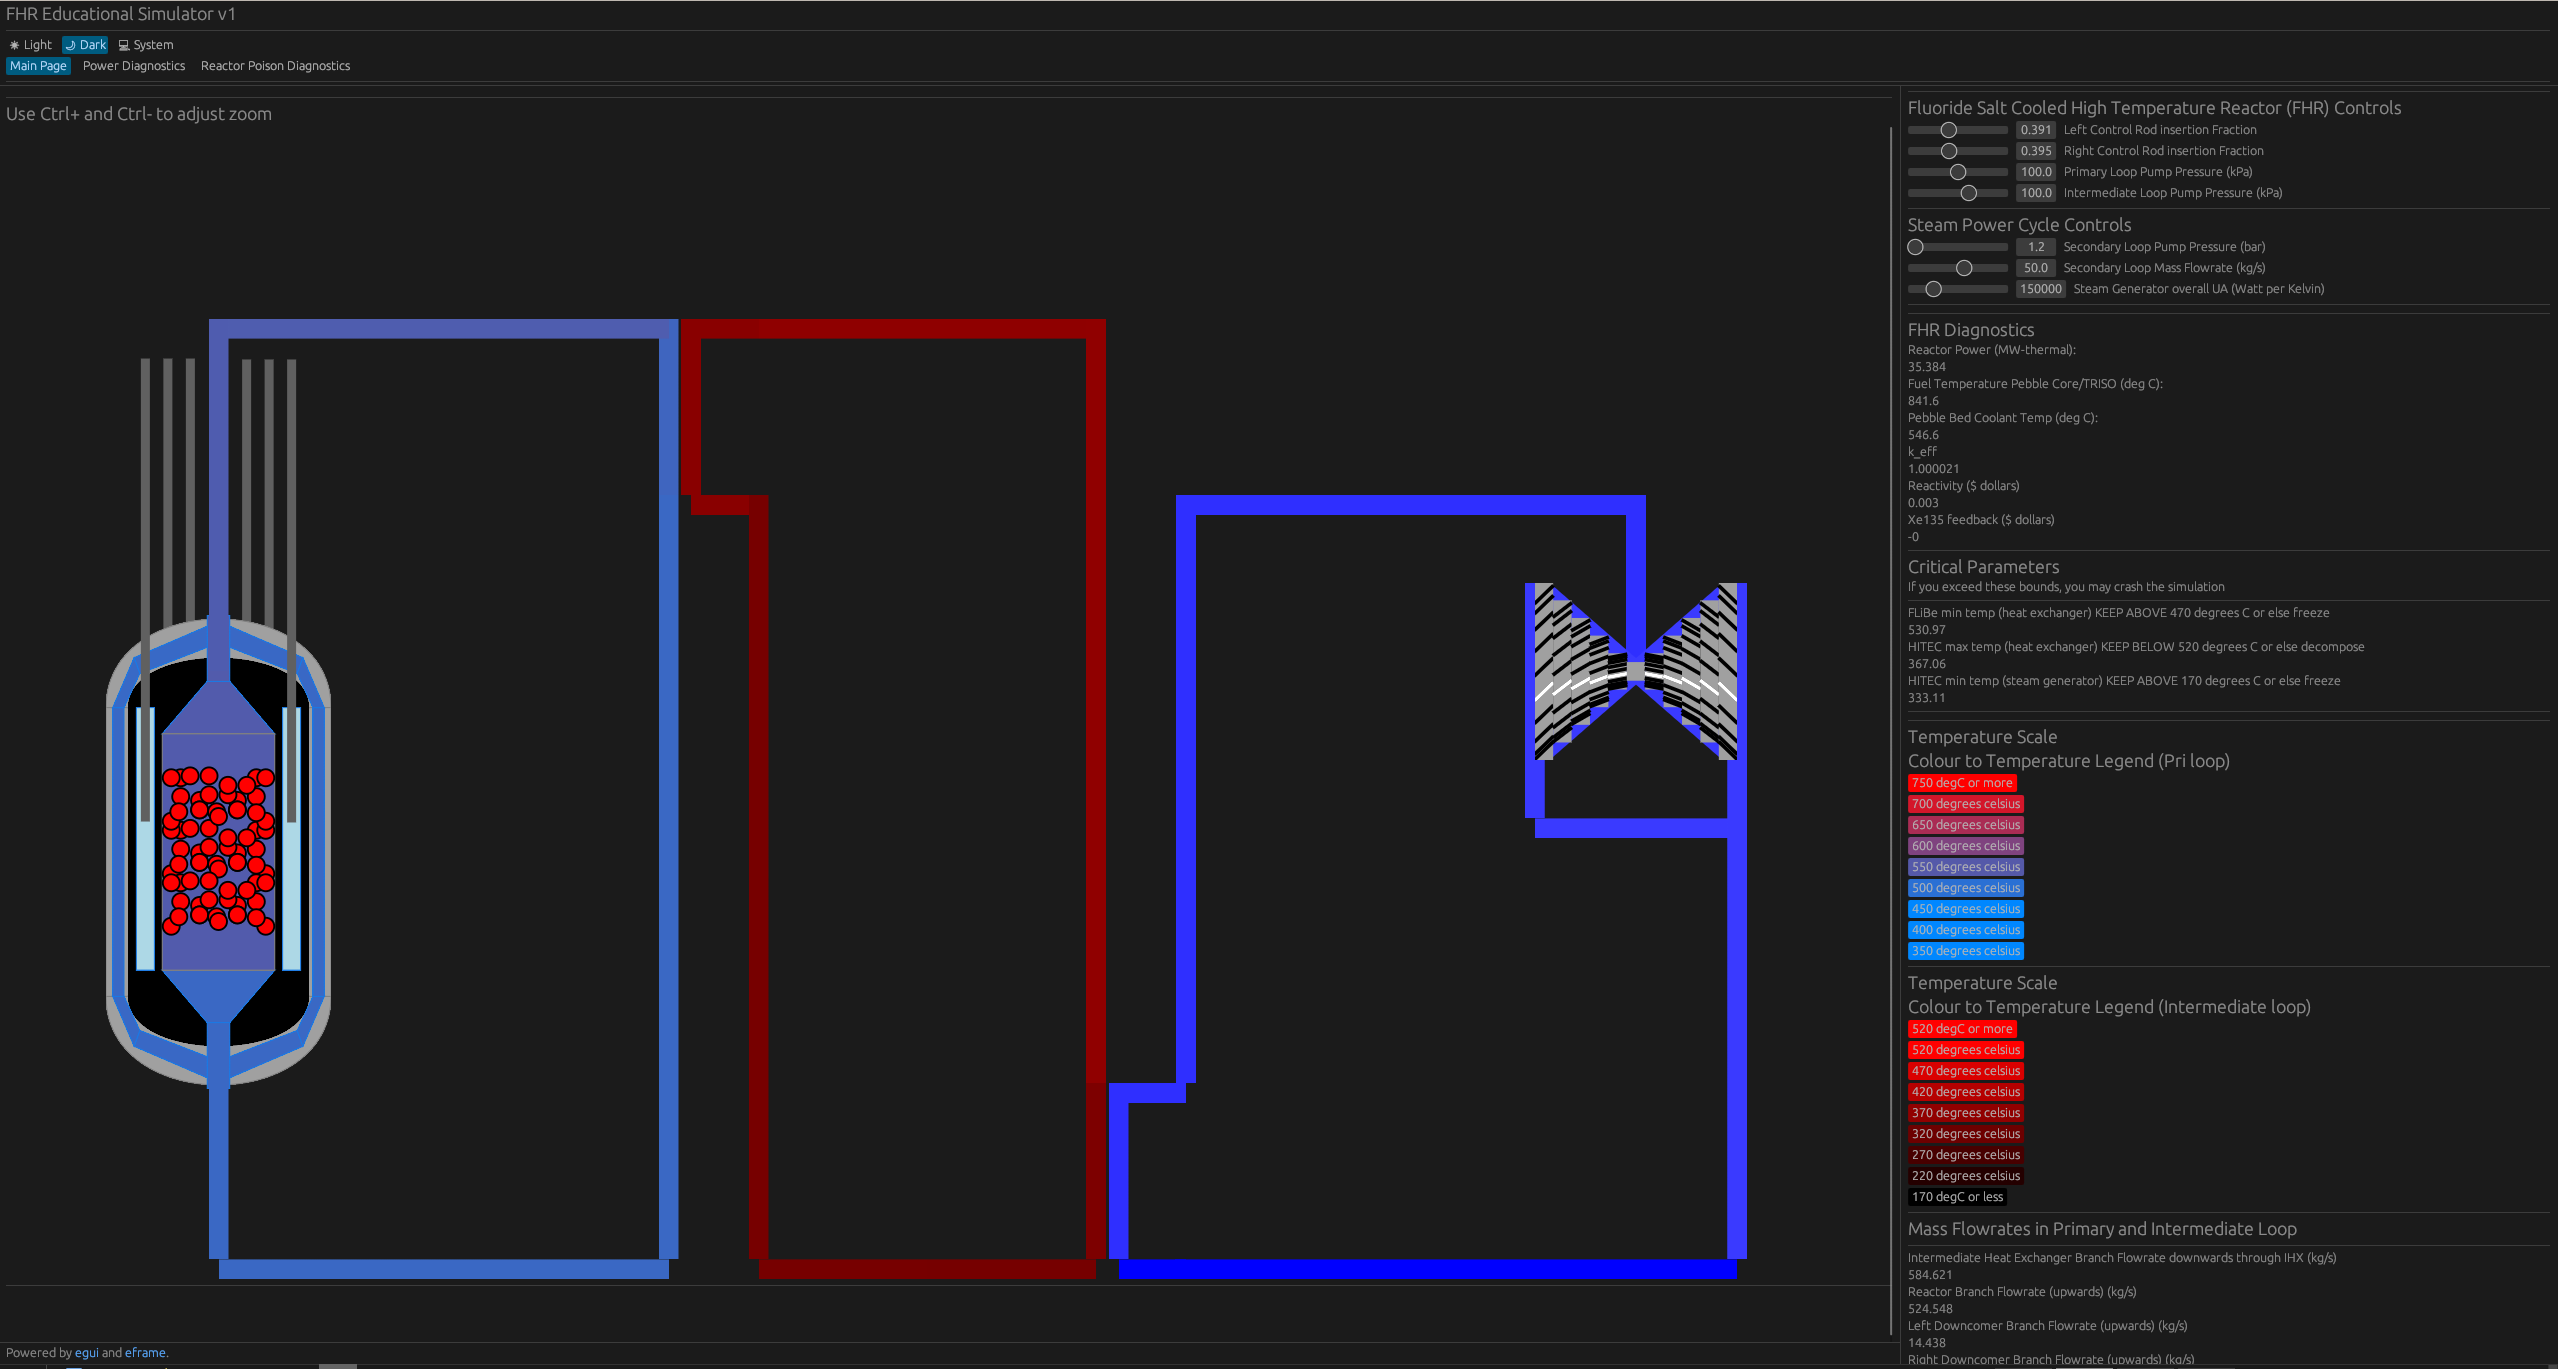
\includegraphics[width=0.7\textwidth, keepaspectratio]{./fhr_sim_full.png}
    \end{figure}
    
    \vspace{1em}
    Looking back at the FHR reactor simulator, hopefully you can now appreciate the deep and complex nuances behind each part of the reactor system.
    
    \vspace{1em}
	\begin{center}
		\textit{Every button, every gauge, and every physical response programmed 
			could not be done without the decades of research into these core phenomena.
		}
    \end{center}
\end{frame}

% =============================================================================
% PART 5: THE CONCLUSION
% =============================================================================

% --- Slide 20: The Call to Adventure ---
\begin{frame}[allowframebreaks]{Your Invitation to the Frontier}
    The journey from a paper design to a safe, working power plant is one of the great engineering challenges of our time.
    
    \vspace{1.5em}
    
    \begin{alertblock}{A Grand Challenge for Singapore}
        We hope that you are interested to study more, and one day help unravel the problem of using nuclear power safely and economically for our nation.
    \end{alertblock}
    
    \vspace{1.5em}
    This field needs bright minds from many disciplines:
    \begin{itemize}
        \item Nuclear Engineers 
        \item Physicists \& Chemists
        \item Mechanical, Electrical, \& Chemical Engineers
        \item Materials Scientists
        \item Computer Scientists \& Software Developers
        \item And many more \dots
    \end{itemize}
\end{frame}

% --- Slide 21: Acknowledgments (Revised) ---
\begin{frame}[allowframebreaks]{Acknowledgments}
    \begin{block}{Development of These Materials}
        This presentation was developed with assistance from \textbf{Google's Gemini model} via \textbf{NUS AI-Know}, the National University of Singapore's trusted generative AI platform \cite{aiknow2025prke}.
    \end{block}

    \vspace{1em}
    \textbf{AI-Know Platform:}
    \begin{itemize}
        \item A secure, compliant AI environment aligned with NUS policies.
        \item Access to leading large language models, including Google's Gemini, for conversational AI and content development.
        \item Private interactions that are never used to train models.
    \end{itemize}

    \vspace{1em}
    \textbf{Special Thanks:}
    \begin{itemize}
        \item NUS SNRSI, for their support in enabling me to develop the simulators used today.
        \item The various historical and technical documentation sources.
    \end{itemize}

    \vspace{1em}
    \centering
    \small
    \textit{For more information about AI-Know: \href{https://ai-know.nus.edu.sg}{https://ai-know.nus.edu.sg}}
\end{frame}

% --- Slide 22: Thank You & References ---
\begin{frame}[allowframebreaks]{Thank You}
    \centering
    \Huge Thank you for your attention.
    
    \vspace{2em}
    \LARGE Questions?
\end{frame}

% --- Slide 23: Bibliography ---
\begin{frame}[allowframebreaks]{References}
    \printbibliography[heading=none]
\end{frame}

\end{document}
